\chapter{Rete di smaltimento delle acque meteoriche allo stato di progetto (con presenza
della rete di drenaggio)} \label{cap:ProgettoRete}
Analizzato quindi il deflusso dei sottobacini presenti nell'area di lavoro, si passa ora alla fase progettuale della rete di drenaggio. 
Tale progettazione sarà suddivisa in tre fasi principali in quanto si è voluto studiare tre casistiche di intervento: una rete di drenaggio composta da sole condotte e tombini, la precedente rete con l'aggiunta di sistemi di laminazione puntuale ed infine l'ulteriore aggiunta di sistemi di laminazione diffusi.

Dato il procedimento iterativo che compone ciascuna fase e il relativo aggiustamento dimensionale delle condotte (dovuto ad esempio  a sottobacini troppo piccoli e verifiche non soddisfatte, ecc) oppure della ri-progettazione della rete con solo i sistemi diffusi (per ottimizzare la dimensione delle condotte) e successiva aggiunta dei sistemi puntuali, si è voluto riportare in questo capitolo solo i risultati delle tre fasi principali sopra descritte e di  riportare invece le fasi intermedie nell'appendice \ref{appendix:FasiIntermedie} a pagina \pageref{appendix:FasiIntermedie}. 

Di seguito verranno dapprima riportati i passaggi che contraddistinguono il dimensionamento e la verifica delle condotte in comune di ciascuna fase, per poi concentrarsi su ciascuna casistica riportando i risultati in forma per lo più tabellare o grafica.

\section{Procedimento per il progetto e verifica}
Data la necessità di conoscere il volume di riempimento delle condotte, la presenza di rigurgito o di moto in pressione è necessario cambiare le modalità di calcolo per la risoluzione della rete.
Nelle ipotesi di moto vario a superficie libera monodimensionale e con condotte di piccola pendenza, gradualmente variato e con fluido incomprimibile si utilizza ora il metodo dell'\emph{Onda Dinamica} che consiste nel considerare tutti i termini dell'equazione di De Saint Venant \ref{eq:saintvenant} relativa alla conservazione della quantità di moto, senza perciò trascurare quelli relativi al gradiente di pressione (come nel metodo dell'\emph{Onda Cinematica} visto prima in cui si era posto $S_0 = S_f$) e i termini inerziali. 
\begin{equation}
    \label{eq:saintvenant}
    \frac{\partial Q}{\partial t} + \frac{\partial}{\partial x} \left( \frac{Q^2}{A} \right) + g A \frac{\partial y}{\partial x} - g A (S_0 - Sf) = 0
 \end{equation}

\subsection{Profondità scavo}
Una volta scelto il percorso delle condotte e dei relativi tombini di collegamento, si deve fare in modo di allineare ciascuna di esse al cielo: 
questo per consuetudine italiana in cui si vuole avere più facilità di manutenzione e di posa degli strati in sommità delle condotte. 
Occorre quindi ipotizzare una pendenza delle condotte $i_G^{prog}$ di primo tentativo e successivamente calcolare la profondità di scavo (\emph{Max Depth}) data dalla differenza tra la quota del terreno e la quota di fondo.
La quota del terreno la si ottiene dai dati altimetrici dell'area (estratti usando QGIS), mentre la quota di fondo è data dalla somma, da valle a monte, dei dislivelli $\Delta h = i_G^{prog} \cdot L_{\text{condotta}}$ di ciascun tratto, partendo dalla quota nota dei recapiti finali (chiamati R1, R2, R3 nelle tabelle e nelle figure che seguiranno d'ora in poi).

Si ottiene così per ogni tratto una \emph{Max Depth} che deve essere
\begin{equation}
    \SI{1.5}{\metre} \lessapprox Max Depth \lessapprox\SI{6.5}{\metre}\quad ,
\end{equation} 
in modo di avere da un lato un ricoprimento minimo delle condotte tale che non si danneggino con il carico di veicoli, persone o intemperie;  dall'altro un ricoprimento contenuto da non avere costi di scavo troppo elevati. 
Per stare all'interno di tale intervallo si va ad agire sulla pendenza di progetto delle condotte o, eventualmente, su sistemi di rinforzo delle stesse.
\subsection{Diametro}
Con le ipotesi di moto sopra dette, si deve progettare la dimensione delle condotte facendo in modo di rispettare il loro riempimento così da rimanere all'interno delle ipotesi. 
Per questo si è imposto un riempimento ideale $\hat{\beta}$ del \SI{75}{\percent}
\begin{equation}
    \hat{\beta} = \frac{h}{d} = \SI{0.75}{}
\end{equation}

Dalla formula di TIZIO applicata al caso di condotte a sezione circolare e in riferimento alla nomenclatura di figura CAIA si ha tale legge che esprime la portata in funzione del riempimento:
\begin{equation}
    Q(\beta) 
    = A(\beta) \, K_S \, R^{\tfrac{2}{3}} \, i^{\tfrac{1}{2}} 
    = \frac{ D \, K_S \, f(\beta)^{\tfrac{5}{3}} \, i^{\tfrac{1}{2}} }{ 2^{\tfrac{13}{3}} \, g(\beta)^{\tfrac{2}{3}} }
\end{equation}
dove 
\begin{align}
    f(\beta) &= \pi - 2 \alpha - 2 (1 - 2 \beta) \cos(\alpha) \\
    g(\beta) &= \pi - 2 \alpha \\
    \alpha &= \arcsin(1 - 2 \beta)
\end{align}
e dalla quale si può ricavare il diametro minimo per il riempimento $\beta = \hat{\beta}$ fissato, avendo nota la portata $Q$ pari al deflusso a monte di tale condotta:
\begin{equation}
    D_{prog}(\hat{\beta}) = \frac{ 2^{\tfrac{13}{8}} \, g(\hat{\beta})^{\tfrac{1}{4}} }{     K_S^{\tfrac{3}{8}} \, f(\hat{\beta})^{\tfrac{5}{8}} } \frac{Q^{\tfrac{3}{8}}}{i^{\tfrac{3}{16}}} \quad .
\end{equation} 

Da tale diametro minimo se ne va a scegliere uno di sezione immediatamente superiore -- o al più di poco inferiore, a causa delle verifiche di riempimento nel capitolo successivo -- disponibile commercialmente.

Infine si calcola per ogni tratto la differenza di dimensione tra la condotta con diametro maggiore e tutte le altre, in modo da inserirle in SWMM e ottenere l'allineamento al cielo.

\subsection{Riporto in SWMM}
\subsection{Verifiche alle condotte}
Il riempimento della condotta $G_\text{cond.}$ deve risultare 
\begin{equation}
    \SI{50}{\percent} \lessapprox G_\text{cond.} \lessapprox\SI{75}{\percent}
\end{equation}


\begin{equation}
    \SI{0.5}{\metre\per\second} < V <  \SI{5}{\metre\per\second}
\end{equation}

Criterio di autopulizia
\begin{equation}
    \tau = \gamma \, R_H \, i_F > \SI{2}{\pascal}
\end{equation}
dove $\gamma$ è il peso specifico dell'acqua pari a \SI{1000}{\newton\per\metre\cubed}, $R_H$ è il raggio idraulico calcolato con la formula di BOH NUM e $i_f$ è la pendenza del fondo vista prima TAB.  
\begin{align}
    R_H &= \frac{D}{4} \, \frac{1 - \sin(\vartheta)}{\vartheta} \\
    \vartheta &= 2 \, \arccos(1 - G_\text{cond.})
\end{align}






\section{Progetto}
Il procedimento sopra descritto è stato pertanto applicato durante il progetto, talvonta iterando i valori quali la ppendenza di progetto i 

come abbiamo scelto il percorso, il Ks, CLS, ogni quanto abbiamo messo i tombini ecc
i problemi con un tombino e la soluzione scelta

\TabellaNodi{Nodi nodes-mod}{tab:Nodi_nodes-mod}{IMG/Nodi-nodes-mod.tex}
\TabellaDiametriCondotte{Diametri progetti conduct-mod}{tab:Diametri_conduct-mod}{IMG/Diametri-conduct-mod.tex}
\TabellaVerificheLinkFLow{Progetto -- Verifiche di massima velocità, riempimento condotta e del criterio di autopulizia}{tab:LinkFlow_Verifiche-MOD}{IMG/LinkFlow-Verifiche-MOD.tex}
\section{Progetto con vasche}
%\chapter{vasche belle  belle}
Al progetto della rete di drenaggio vengono ora aggiunte tre vasche di laminazione in corrispondenza dei tre sbocchi della rete e chiamate rispettivamente: \emph{Nord}, \emph{Centro} e \emph{Sud}.
Lo scopo di tali vasche è quello di fungere da ammortizzatore idraulico venendo dimensionate in modo da contenere la portata massima scaricata nel corpo idrico recettore.

Il predimensionamento delle vasche si articola in un metodo iterativo per far sì di avere il maggior riempimento di esse (prossimo al \SI{100}{\percent}) e parallelamente un \emph{Maximum Outflow} minore della massima portata da mantenere come da progetto. 
Tale portata è calcolata tenendo conte delle prescrizioni legislative per il coefficiente udometrico, che per Trento è pari a $C_{udo} = \SI{20}{\litre\per\second\per\hectare}$, fissando così la portata massima in uscita da scaricare. 

La portata massima da mantenere pertanto diviene:
\begin{equation}
    Q_{max} = C_{udo} \cdot A_{\text{sottobacino}}
    \label{eq:qmax} \quad ,
\end{equation}
dove con $A_{\text{sottobacino}}$ si intende l'area di pertinenza di ciascuna vasca, ovvero la somma delle aree dei sottobacini confluenti in essa.

I parametri da variare nell'iterazione (in fase non esecutiva del progetto) sono l'area della vasca e il diametro dell'orifizio della stessa (o analogamente l'area dell'orifizio -- essendo di sezione cilindrica). 


Come prima iterazione l'area dell'orifizio è calcolata invertendo la formula della forometria della portata uscente e ponendola uguale alla $Q_{max}$:
\begin{equation}
    Q  = C_{eff} A_{\text{orifizio}} \sqrt{2 g h} \overset{!}{=} Q_{max} \quad .
\end{equation}
Si è scelto un coefficiente di efflusso $C_{eff} = \SI{0.65}{}$, avendo una bocca a battente a luce fissa e verticale. 
Mentre l'area della vasca è calcolata dividendo il volume totale da invasare per la profondità della vasca di progetto $h = \SI{1.50}{\metre}$.

Il volume totale da invasare è stato calcolato come sommatoria dell'area compresa tra le due curve (visibili in figura \ref{fig:vasche}) corrispondenti al deflusso nella condotta senza vasca e al deflusso attenuato dalla presenza della vasca. 
Le funzioni delle curve sono state discretizzate con un intervallo di 60 secondi e la parte compresa tra loro è stata calcolata come differenza delle due aree sottese e ottenute tramite il metodo dei trapezi.
\begin{figure}[p]
    \centering
    \begin{tikzpicture}
        \begin{axis}[
            %restrict x to domain=-0:1.5,
            height=6.5cm,
            width=15cm,
            grid=major,
            %xlabel=Tempo trascorso dall'inizio della precipitazione \si{[\hour]},
            ylabel=Deflusso  \si{[\litre\per\second]},
            xtick = {0,0.5,1,1.5,2,2.5,3,3.5,4},
            title= \emph{Vasca 1 posta a monte della condotta C11},
            /pgf/number format/.cd,
            use comma,
            1000 sep={\,}
        ]
        \addplot +[mark=none,style=solid,color=blue] table[x index=0,y index=1,header=false] {IMG/vasche/vasca1.txt};
        \addplot +[mark=none,style=solid,color=orange] table[x index=0,y index=2,header=false] {IMG/vasche/vasca1.txt};
        \node at (axis cs:1.4,160) [anchor=south west] {\SI{164.51}{\litre\per\second}};
        \legend{Pre vasca, Post vasca}    
        \end{axis}
    \end{tikzpicture}

    \vspace{.5cm}
    %
    \begin{tikzpicture}
        \begin{axis}[
            %restrict x to domain=-0:1.5,
            height=6.5cm,
            width=15cm,
            grid=major,
            %xlabel=Tempo trascorso dall'inizio della precipitazione \si{[\hour]},
            ylabel=Deflusso  \si{[\litre\per\second]},
            xtick = {0,0.5,1,1.5,2,2.5,3,3.5,4},
            title= \emph{Vasca 2 posta a monte della condotta C21} ,
            /pgf/number format/.cd,
            use comma,
            1000 sep={\,}
        ]
        \addplot +[mark=none,style=solid,color=blue] table[x index=0,y index=1,header=false] {IMG/vasche/vasca2.txt};
        \addplot +[mark=none,style=solid,color=orange] table[x index=0,y index=2,header=false] {IMG/vasche/vasca2.txt};
        \node at (axis cs:1.4,70) [anchor=south west] {\SI{57.30}{\litre\per\second}};
        \legend{Pre vasca, Post vasca}    
        \end{axis}
    \end{tikzpicture}

    \vspace{.5cm}
    %
    \begin{tikzpicture}
        \begin{axis}[
            %restrict x to domain=-0:1.5,
            height=6.5cm,
            width=15cm,
            grid=major,
            xlabel=Tempo trascorso dall'inizio della precipitazione \si{[\hour]},
            ylabel=Deflusso  \si{[\litre\per\second]},
            xtick = {0,0.5,1,1.5,2,2.5,3,3.5,4},
            title= \emph{Vasca 3 posta a monte della condotta C29},
            /pgf/number format/.cd,
            use comma,
            1000 sep={\,}
        ]
        \addplot +[mark=none,style=solid,color=blue] table[x index=0,y index=1,header=false] {IMG/vasche/vasca3.txt};
        \addplot +[mark=none,style=solid,color=orange] table[x index=0,y index=2,header=false] {IMG/vasche/vasca3.txt};
        \node at (axis cs:1.4,160) [anchor=south west] {\SI{147.66}{\litre\per\second}};
        \legend{Pre vasca, Post vasca}    
        \end{axis}
    \end{tikzpicture}
    %
    \caption{Attenuazione del deflusso nelle tre condotte con l'introduzione delle vasche a monte delle condotte}
    \label{fig:vasche}
\end{figure}
%%%%%%%%%%%%%%%%%%%%%%%%%%%%
L'attenuazione del deflusso è stata calcolata partendo dalla $Q_{max}$ trovata nella formula \ref{eq:qmax} ed utilizzando la seguente legge
\begin{equation}   
    Q_{OUTflow}= 
    \begin{cases}
        Q_{INflow} & \text{se $Q_{INflow} \leq Q_{max}$}\\
        Q_{max} & \text{se $Q_{INflow} > Q_{max}$}\\
    \end{cases}
\end{equation}

I dati progettuali ottenuti con le considerazioni appena viste sono riportati in tabella \ref{tab:datiProgettoVasche}.
\begin{table}[htb] 
    \centering
    \caption{Parametri per il progetto della vasca di laminazione}
    \label{tab:datiProgettoVasche}
    \begin{tabular}{lS[table-format=3.2]S[table-format=3.2]S[table-format=3.2]}
        \toprule
                                & \multicolumn{1}{c}{Nord}   & \multicolumn{1}{c}{Centro} & \multicolumn{1}{c}{Sud}    \\
        \midrule
        Area pertinenza vasca \si{[\hectare]} & 8.23   & 2.87  & 7.38   \\
        $Q_{max}$ \si{[\litre\per\second]}    & 164.51 & 57.30 & 147.66 \\
        Volume da invasare\si{[\metre\cubed]} & 229.59 & 65.47 & 366.12 \\
        Area vasca \si{[\square\metre]}       & 153.06 & 43.65 & 244.08 \\
        Area orifizio \si{[\square\metre]}    & 0.05   & 0.02  & 0.04   \\
        Diametro orifizio   \si{[\metre]}     & 0.24   & 0.14  & 0.23   \\
        \bottomrule
\end{tabular}%
\end{table}

In tabella \ref{tab:iterazioni} sono riportate le varie iterazioni per ciascuna vasca  e con il grassetto si intende il valore di fine iterazione scelto. 
Per questi sono inoltre riportati i restanti  parametri  della vasca ovvero il volume medio e il volume massimo di riempimento.
\begin{table}[htb] 
    \centering
    \caption{Iterazioni dell'Altezza dell'orifizio e dell'Area della vasca per avere il massimo riempimento della vasca e mantenere la portata inferiore a quella massima. In grassetto sono indicate le scelte}
    \label{tab:iterazioni}
    \begin{tabular}{cS[table-format=1.2]S[table-format=3.0]S[table-format=3.0]S[table-format=3.2]}
        \toprule
                            & \multicolumn{1}{c}{Altezza \si{[\metre]}}    & \multicolumn{1}{c}{Area vasca \si{[\square\metre]}} & \multicolumn{1}{c}{\si{\percent} riempimento max} & \multicolumn{1}{c}{ Deflusso max \si{[\litre\per\second]}} \\
                            \midrule
    \multirow{5}{*}{Nord}   & 0.24    & 155    & 100 & 152.4            \\
                            & 0.24    & 180    & 100 & 152.4            \\
                            & 0.24    & 200    & 100 & 152.4          \\
                            & \B 0.24 & \B 210 & 97  & 150.15           \\
                            & 0.25    & 210    & 94  & 159.59            \\
                            \midrule
    \multirow{3}{*}{Centro} & 0.14    & 45     & 100 & 52.79            \\
                            & \B 0.14 & \B 60  & 94  & 51.15            \\
                            & 0.14    & 55     & 99  & 52.53            \\
                            \midrule
    \multirow{5}{*}{Sud}    & 0.23    & 245    & 100 & 140.22           \\
                            & 0.23    & 260    & 100 & 140.22           \\
                            & 0.23    & 300    & 100 & 140.22           \\
                            & 0.23    & 350    & 91  & 132.97           \\
                            & \B 0.23 & \B 325 & 95  & 136.43           \\
                            \bottomrule 
    \end{tabular}%
\end{table}

In figura \ref{fig:volume} si confronta il deflusso allo sbocco delle tre reti di drenaggio con e senza vasca di laminazione, graficando l'andamento del volume d'acqua all'interno della vasca.
Si può notare come nel caso di presenza della vasca, l'accumulo di acqua in essa contenuta faccia sì che diminuisca la portata defluita allo sbocco, ritardando inoltre il tempo di massimo deflusso. 
\begin{figure}[p]
    \centering
    \begin{tikzpicture}
        \begin{axis}[
            restrict x to domain=-0:6,
            height=6.5cm,
            width=15cm,
            grid=major,
            %xlabel=Tempo trascorso dall'inizio della precipitazione \si{[\hour]},
            ylabel=Deflusso  \si{[\litre\per\second]} e Volume  \si{[\metre\cubed]},
            xtick = {0,0.5,1,1.5,2,2.5,3,3.5,4,4.5,5,5.5,6},
            title= \emph{Vasca 1 posta a monte della condotta C11},
            /pgf/number format/.cd,
            use comma,
            1000 sep={\,}
        ]
        \addplot +[mark=none,style=solid,color=red] table[x index=0,y index=1,header=false] {IMG/vasche/Volume1.txt};
        \addplot +[mark=none,style=solid,color=blue] table[x index=0,y index=1,header=false] {IMG/vasche/vasca1.txt};
        \addplot +[mark=none,style=solid,color=cyan] table[x index=0,y index=1,header=false] {IMG/vasche/Inflow1.txt};
        
        \legend{Volume vasca, Deflusso pre vasca, Deflusso post vasca }    
        \end{axis}
    \end{tikzpicture}

    \vspace{.5cm}
    %
    \begin{tikzpicture}
        \begin{axis}[
            restrict x to domain=-0:6,
            height=6.5cm,
            width=15cm,
            grid=major,
            %xlabel=Tempo trascorso dall'inizio della precipitazione \si{[\hour]},
            ylabel=Deflusso  \si{[\litre\per\second]} e Volume  \si{[\metre\cubed]},
            xtick = {0,0.5,1,1.5,2,2.5,3,3.5,4,4.5,5,5.5,6},
            title= \emph{Vasca 2 posta a monte della condotta C21},
            /pgf/number format/.cd,
            use comma,
            1000 sep={\,}
        ]
        \addplot +[mark=none,style=solid,color=red] table[x index=0,y index=1,header=false] {IMG/vasche/Volume2.txt};
        \addplot +[mark=none,style=solid,color=blue] table[x index=0,y index=1,header=false] {IMG/vasche/vasca2.txt};
        \addplot +[mark=none,style=solid,color=cyan] table[x index=0,y index=1,header=false] {IMG/vasche/Inflow2.txt};
        
        \legend{Volume vasca, Deflusso pre vasca, Deflusso post vasca }    
        \end{axis}
    \end{tikzpicture}

    \vspace{.5cm}
    %
    \begin{tikzpicture}
        \begin{axis}[
            restrict x to domain=-0:6,
            height=6.5cm,
            width=15cm,
            grid=major,
            xlabel=Tempo trascorso dall'inizio della precipitazione \si{[\hour]},
            ylabel=Deflusso  \si{[\litre\per\second]} e Volume  \si{[\metre\cubed]},
            xtick = {0,0.5,1,1.5,2,2.5,3,3.5,4,4.5,5,5.5,6},
            title= \emph{Vasca 3 posta a monte della condotta C29},
            /pgf/number format/.cd,
            use comma,
            1000 sep={\,}
        ]
        \addplot +[mark=none,style=solid,color=red] table[x index=0,y index=1,header=false] {IMG/vasche/Volume3.txt};
        \addplot +[mark=none,style=solid,color=blue] table[x index=0,y index=1,header=false] {IMG/vasche/vasca3.txt};
        \addplot +[mark=none,style=solid,color=cyan] table[x index=0,y index=1,header=false] {IMG/vasche/Inflow3.txt};
        
        \legend{Volume vasca, Deflusso pre vasca, Deflusso post vasca }    
        \end{axis}
    \end{tikzpicture}
    %
    \caption{Confronto del deflusso allo sbocco della rete pre e post l'installazione delle vasche e andamento del volume d'acqua all'interno delle stesse}
    \label{fig:volume}
\end{figure}


\section{Progetto con vasche e lid}
DA SISTEMARE IL CONDUCT2
\TabellaDiametriCondotte{Diametri progetti conduct2}{tab:Diametri_Conduct2}{IMG/Diametri-Conduct2.tex}



\appendix
\chapter{ROBE DA SWMM}
\label{appendix:SWMM}
%
\begin{figure}[htbp]
    \centering
    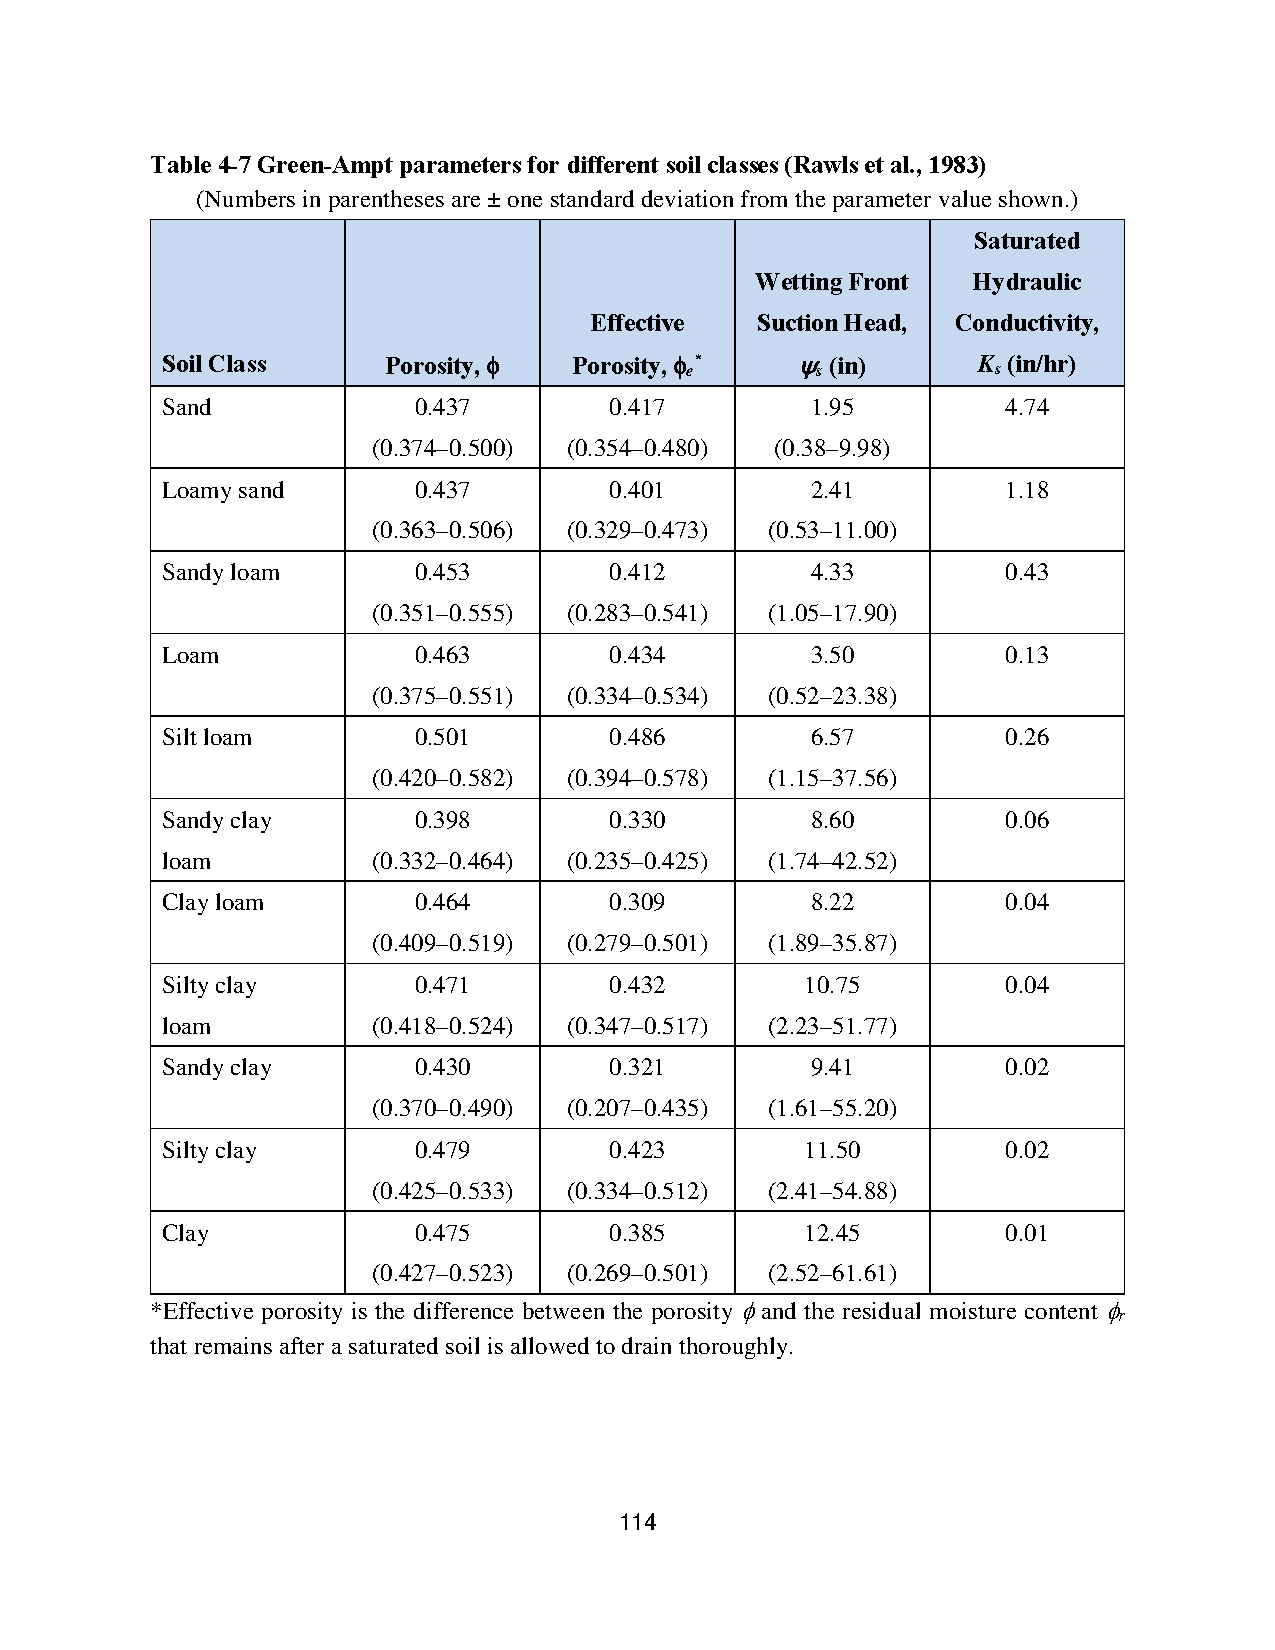
\includegraphics[trim=2.5cm 4.5cm 2.5cm 3.6cm,clip,width=\textwidth]{IMG/table4-7_Ks.pdf} 
    \caption[Tabella 4.7 di SWMM]{Tabella 4.7 di SWMM Green-Ampt parameters for different soil classes (Rawls et al., 1983) (Numbers in parentheses are ± one standard deviation from the parameter value shown.)}
    \label{SWMM:tabella4-7}
\end{figure}

\chapter{Rete di smaltimento delle acque meteoriche allo stato di progetto (con presenza
della rete di drenaggio) - tutti i mancanti}
\label{appendix:FasiIntermedie}
\section{Progetto sbagliato}
\section{Progetto con solo i LID}
\TabellaDiametriCondotte{Diametri progetti conduct-mod LID. In verde sono indicati i valori che hanno subito una modifica rispetto al progetto senza LID}{tab:Diametri_conduct-mod-LID}{IMG/Diametri-conduct-mod-LID.tex}
\TabellaVerificheLinkFLow{Progetto con aggiunta dei soli LID -- Verifiche di massima velocità, riempimento condotta e del criterio di autopulizia}{tab:LinkFlow_Verifiche-MOD-LID}{IMG/LinkFlow-Verifiche-MOD-LID.tex}
\section{Progetto con vasche e lid rifatto dopo i lid}
\section{Progetto con vasche e lid sistemato}
